\section{Introducción}
\textbf{Parrafo sin corregir:} El signo de Hoffmann es un reflejo muscular que se produce al percutir suavemente el lecho ungueal del dedo medio o índice, como se muestra en la figura \ref{fig:Hoffmann_sign}, produciéndose un movimiento de flexión involuntario del pulgar cuando el examinador hace girar la uña del dedo medio hacia abajo. Fue propuesto por primera vez por Johann Hoffmann, un neurólogo alemán, a finales del siglo XIX, y descrito por primera vez por Hans Curschmann, uno de sus asistentes, en 1911 \cite{BENDHEIM}. El signo de Hoffmann también ha sido denominado de diferentes formas, como 'reflejo digital', 'reflejo de chasquido', 'signo de Tromner' y 'signo de Jakobson' \cite{glaser2001cervical}.


\textbf{Parrafo Corregido:} El signo de Hoffmann es un reflejo patológico que se desencadena al percutir la uña del dedo medio, produciéndose un movimiento de flexión involuntario del pulgar cuando el examinador mueve la uña del dedo medio hacia abajo (ver Figur \ref{fig:Hoffmann_sign}). Fue propuesto por el neurólogo alemán Johann Hoffmann, a finales del siglo XIX, y descrito por primera vez por su asistente Hans Curschmann, en 1911 \cite{BENDHEIM}. El signo de Hoffmann también ha sido denominado de diferentes formas, como 'reflejo digital', 'signo de Jakobson', entre otros \cite{glaser2001cervical}.

\begin{figure}[h!]
	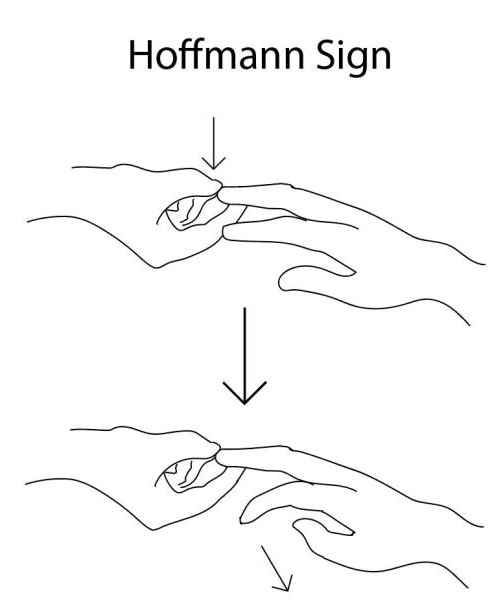
\includegraphics[width=0.35\textwidth]{figures/Kabir_Hoffmann__Sign.jpg}
	\caption{Signo de Hoffmann. Este diagrama muestra un signo de Hoffmann positivo, una parte estándar del examen neurológico común. Contribución de R Kabir, MD}
	\label{fig:Hoffmann_sign}
\end{figure}

Se ha utilizado en la práctica clínica durante aproximadamente cien años como una herramienta para detectar alteraciones en las vías corticoespinales, las cuales conectan la corteza cerebral con la médula espinal. Estudios realizados en la década de 1930 evaluaron la incidencia del signo en estudiantes universitarios sanos, encontrando una incidencia del 2\% y 1.63\% \cite{echols1936hoffmann} \cite{fay1933clinical}, respectivamente, aunque solo se incluyeron sujetos masculinos \cite{glaser2001cervical}. Este hallazgo clínico ha sido útil en la detección de mielopatía cervical espondilótica temprana \cite{denno1991early}, como lo propusieron Denno y Meadows al describir el signo de Hoffmann 'dinámico', una variante de la prueba con flexiones activas del cuello \cite{glaser2001cervical}.

Es importante destacar que el signo de Hoffmann es un fenotipo y no una enfermedad en sí, ya que se ha descubierto que hasta el 3\% de la población presenta un signo de Hoffmann positivo sin que haya compresión de la médula. Este fenotipo actualmente está asociado a 12 enfermedades diferentes \cite{whitney}.

El signo de Hoffmann ha sido identificado en una serie de enfermedades neurodegenerativas y trastornos del tracto corticoespinal, muchas de ellas caracterizadas por alteraciones motoras progresivas. Entre estas patologías se encuentran diversas formas de paraplejía espástica hereditaria. Estas son un grupo clínicamente y genéticamente heterogéneo de trastornos neurológicos, caracterizados principalmente por espasticidad progresiva y, a menudo, pérdida del sentido de la vibración en los miembros inferiores \cite{Esteves2014}, tanto autosómica dominante como recesiva. Por ejemplo, la paraplejía espástica 9A, de herencia autosómica dominante \cite{10.1093/brain/awv143}, y las formas recesivas como la paraplejía espástica 72, asociadas con disfunción motora grave.

Enfermedades neurodegenerativas más conocidas, como la esclerosis lateral amiotrófica (ELA), también muestran una asociación con el signo de Hoffmann, debido a la degeneración de las motoneuronas superiores \cite{RIANCHO201927}. Diversas formas de ataxias espásticas, relacionadas con la falta de coordinación motora \cite{Pedroso2022}, como la ataxia espástica 9 y 10, completan el espectro de condiciones en las que este reflejo patológico se manifiesta.

\begin{table}[h!]
	\centering
	\caption{Lista de enfermedades con sus respectivos identificadores de las bases de datos Online Mendelian Inheritance in Man (OMIM)\cite{omim} y Online Database of Rare Diseases and Orphan Drugs (ORPHA)\cite{orphanet}.}
	\setlength{\extrarowheight}{2pt}
	\begin{tabular}{|>{\centering\arraybackslash}m{3cm}|>{\raggedright\arraybackslash}m{10cm}|}
		\hline
		\textbf{Disease Id}  & \textbf{Disease Name} \\ \hline
		OMIM:601162          & Spastic paraplegia 9A, autosomal dominant \\ \hline
		OMIM:618850          & Hypervalinemia or hyperleucine-isoleucinemia \\ \hline
		ORPHA:206448         & Adult Krabbe disease \\ \hline
		OMIM:615625          & Spastic paraplegia 72, autosomal recessive \\ \hline
		ORPHA:803            & Amyotrophic lateral sclerosis \\ \hline
		OMIM:620402          & Neuronopathy, distal hereditary motor, autosomal recessive 9 \\ \hline
		OMIM:615491          & Spastic paraplegia 79, autosomal recessive \\ \hline
		OMIM:615681          & Spastic paraplegia 62, autosomal recessive \\ \hline
		ORPHA:139396         & X-linked cerebral adrenoleukodystrophy \\ \hline
		OMIM:620666          & Spastic ataxia 10, autosomal recessive \\ \hline
		OMIM:618438          & Spastic ataxia 9, autosomal recessive \\ \hline
		OMIM:619621          & Spastic paraplegia 84, autosomal recessive \\ \hline
	\end{tabular}
	\label{tab:disease_list}
\end{table}

A nivel molecular, diversos genes han sido asociados con condiciones que incluyen este signo, reflejo que indica alteraciones en los tractos corticoespinales. Entre estos genes destacan SOD1, TARDBP, UBQLN2 y NEK1, todos vinculados a la esclerosis lateral amiotrófica. Las mutaciones en SOD1 \cite{zhao2022g41d}, TARDBP \cite{sanchez2022atypical} y UBQLN2 \cite{teyssou:hal-03001781} afectan las motoneuronas superiores, contribuyendo a la aparición de reflejos patológicos como el signo de Hoffmann. Además, NEK1 ha sido recientemente asociado con formas hereditarias de ELA \cite{mann2023NEK1}, lo que refuerza su implicación en el deterioro de las vías motoras. Las alteraciones en estos genes provocan una degeneración progresiva de las neuronas motoras, subrayando la relevancia del signo de Hoffmann como un marcador clínico clave en enfermedades neurodegenerativas.








